%%%%%%%%%%%%%%%%%%%%%%%%%%%%%%%%%%%%%%%%%%%%%%%%%%%%%%%%%%%%%%%%%%%%%%%%%%%
%
% Template for a LaTex article in English.
%
%%%%%%%%%%%%%%%%%%%%%%%%%%%%%%%%%%%%%%%%%%%%%%%%%%%%%%%%%%%%%%%%%%%%%%%%%%%

\documentclass{article}

% AMS packages:
\usepackage{amsmath, amsthm, amsfonts}
\usepackage{algorithm}
\usepackage[hyperref, UTF8]{ctex}
\usepackage[noend]{algpseudocode}
\usepackage{graphicx}
\usepackage{subcaption}
\usepackage[top=0.8in, bottom=0.8in, left=1in, right=1in]{geometry}
\graphicspath{ {images/} }

% Theorems
%-----------------------------------------------------------------
\newtheorem{thm}{Theorem}[section]
\newtheorem{cor}[thm]{Corollary}
\newtheorem{lem}[thm]{Lemma}
\newtheorem{prop}[thm]{Proposition}
\theoremstyle{definition}
\newtheorem{defn}[thm]{Definition}
\theoremstyle{remark}
\newtheorem{rem}[thm]{Remark}

\makeatletter
\def\BState{\State\hskip-\ALG@thistlm}
\makeatother
%\newcommand*{\rom}[1]{\expandafter\@slowromancap\romannumeral #1@}
\newcommand{\rom}[1]{\uppercase\expandafter{\romannumeral #1\relax}}
% Shortcuts.
% One can define new commands to shorten frequently used
% constructions. As an example, this defines the R and Z used
% for the real and integer numbers.
%-----------------------------------------------------------------
\def\RR{\mathbb{R}}
\def\ZZ{\mathbb{Z}}

% Similarly, one can define commands that take arguments. In this
% example we define a command for the absolute value.
% -----------------------------------------------------------------
\newcommand{\abs}[1]{\left\vert#1\right\vert}

% Operators
% New operators must defined as such to have them typeset
% correctly. As an example we define the Jacobian:
% -----------------------------------------------------------------
\DeclareMathOperator{\Jac}{Jac}

%-----------------------------------------------------------------
\title{Report of paper (Isotopic Approximation within a Tolerance Volume)}
\author{张胜威\\
  %% \small Dept. Templates and Editors\\
  %% \small E12345\\
  %% \small Spain
}

\begin{document}
\maketitle

%% \abstract{Compiling Embedded\_thin\_shell progress}
\section{Bad 3d delaunay triangulation}
  \begin{figure}[h]
    \begin{subfigure}[b]{0.4\textwidth}
      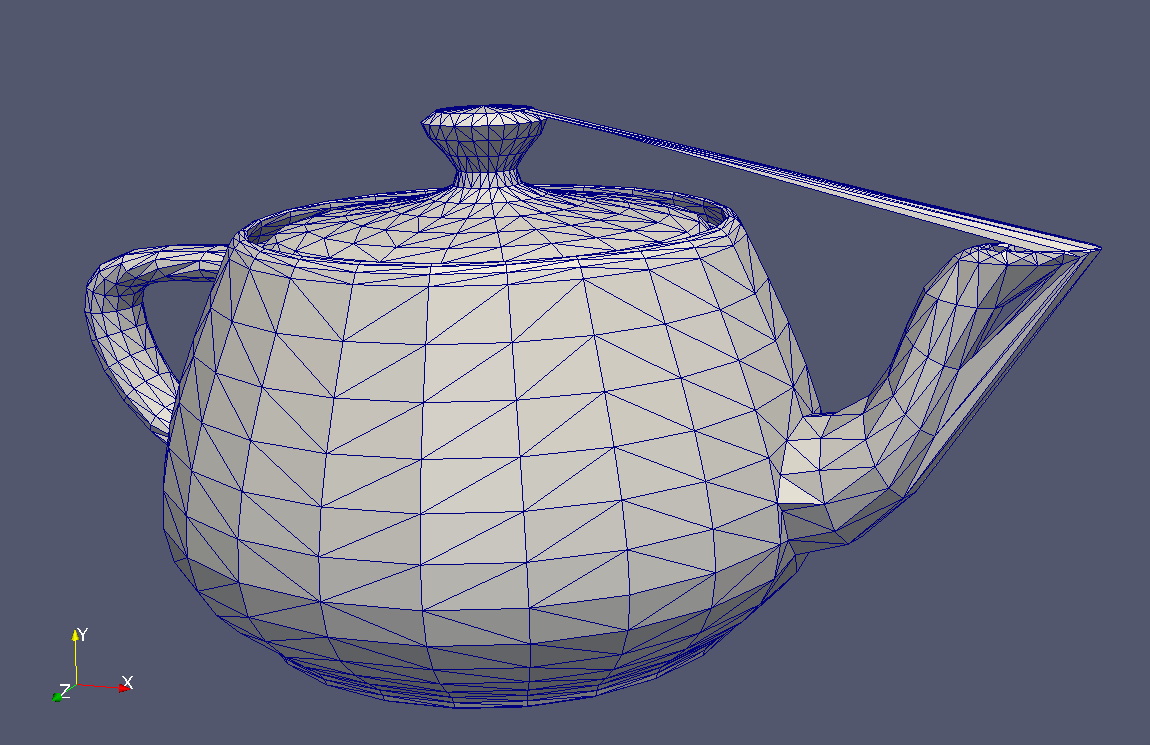
\includegraphics[width=\textwidth]{bad_surface0.png}
      \caption[现象]{bi+zero\_surface的四面体化}
    \end{subfigure}
    \begin{subfigure}[b]{0.4\textwidth}
      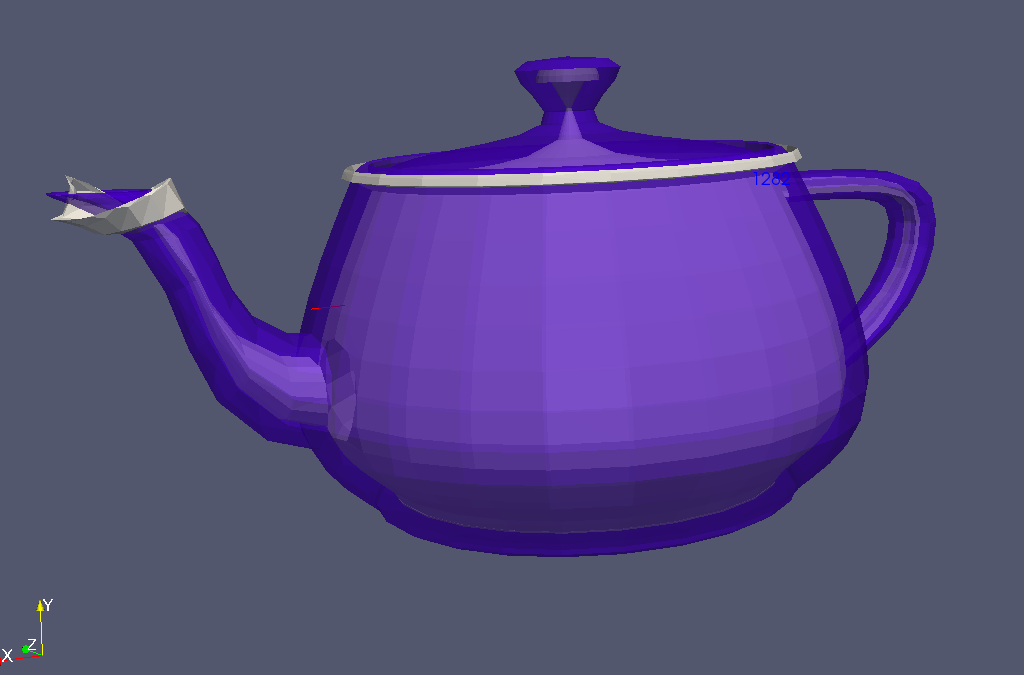
\includegraphics[width=\textwidth]{bad_surface1.png}
      \caption[原因]{zero\_surface和bi相交}
    \end{subfigure}
  \end{figure}

  \begin{figure}
    \begin{subfigure}[b]{0.4\textwidth}
      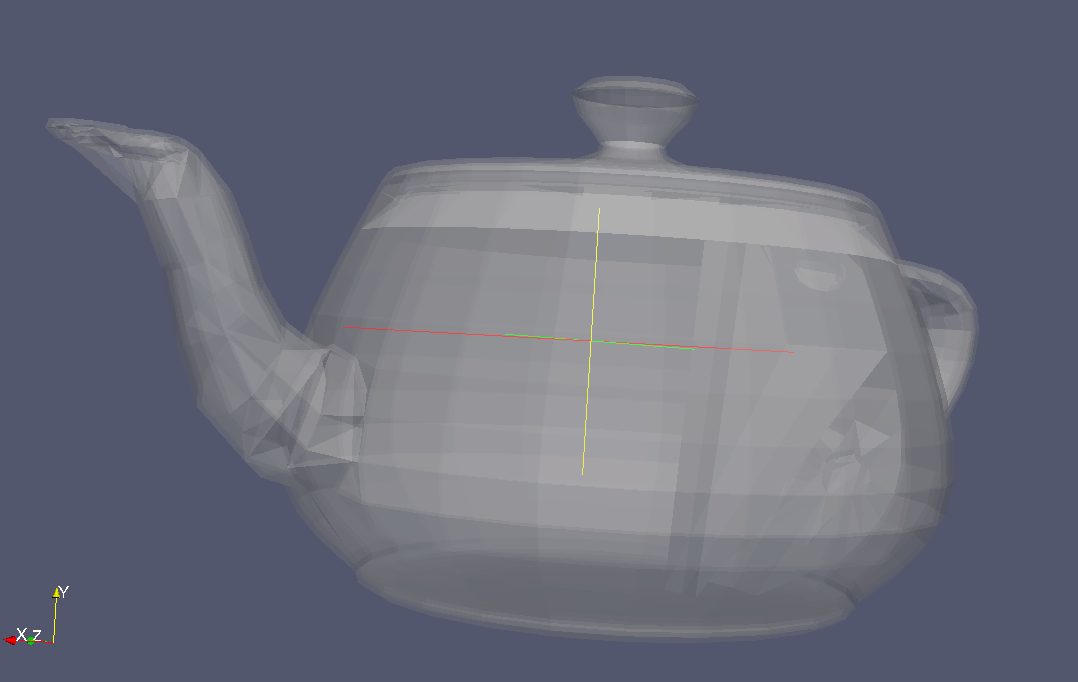
\includegraphics[width=\textwidth]{bad_inner_space0.png}
      \caption[现象]{bo+zero\_surface的四面体化}
    \end{subfigure}
    \begin{subfigure}[b]{0.4\textwidth}
      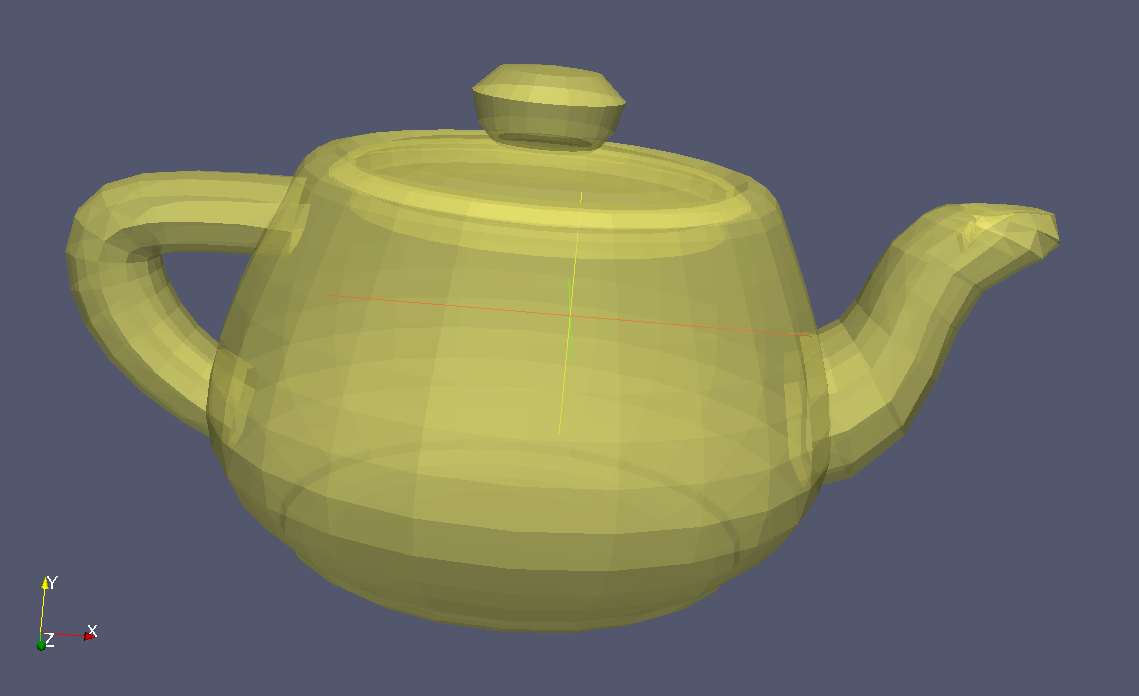
\includegraphics[width=\textwidth]{bad_inner_space1.png}
      \caption[原因]{bad inner space:teaport不连续,有洞}
    \end{subfigure}
  \end{figure}
  理想情况下是:根据原模型(zero\_surface)做生成内外壳,并在保存内外壳的三角化的情况下做一个delaunay triangulation.
  我原来的做法是:(外壳+zero\_surface) + (内壳+zero\_surface).
\end{document}
